\documentclass[conference]{IEEEtran}
\IEEEoverridecommandlockouts
% The preceding line is only needed to identify funding in the first footnote. If that is unneeded, please comment it out.
\usepackage{cite}
\usepackage{amsmath,amssymb,amsfonts}
\usepackage{algorithmic}
\usepackage{graphicx}
\usepackage{textcomp}
\usepackage{xcolor}
\usepackage{float}
\def\BibTeX{{\rm B\kern-.05em{\sc i\kern-.025em b}\kern-.08em
    T\kern-.1667em\lower.7ex\hbox{E}\kern-.125emX}}
\begin{document}

\title{ECE-718: An Extensible Architecture for Hyperdimensional Computing}

\author{\IEEEauthorblockN{1\textsuperscript{st} Graham Power}
\IEEEauthorblockA{\textit{Electrical \& Computer Engineering} \\
\textit{McMaster University}\\
Hamilton, Canada \\
powerg@mcmaster.ca}
}

\maketitle

%\begin{abstract}
%Not using this yet...
%\end{abstract}

%\begin{IEEEkeywords}
%Also not usingthis yet...
%\end{IEEEkeywords}

\section{Introduction}

Hyperdimensional computing is an encoding which stores data in very high dimensional vectors, on the order of thousands to tens of thousands of dimensions. While there are many different ways to represent these vectors \cite{hdccompare}, called encodings, these encodings generally support three fundamental operations. Similarity, a method for comparing two vectors to determine their elements' similarity, generally produces a number bounded of [-1,1]. Bundling, which takes two or more vectors and produces a vector similar to all the inputs, as defined by the similarity metric. Binding, which takes two vectors and produces a vector dissimilar to all the inputs, again as defined by the similarity metric. Usually, binding is commutative and invertible, though there are some exceptions. In VTB\cite{vtb}, MBAT\cite{mbat}, and BSDC-S\cite{bsdc}, binding is not commutative. In HRR\cite{hrr}, MBAT\cite{mbat}, and VTB\cite{vtb} binding is only pseudo-invertable, and in BSDC-CDT\cite{bsdc} binding is entirely non-invertable.

\subsection{The Problem}

While many previous works have implemented HDC accelerators \cite{rischd, sparsehd, bric}, they have all been restricted to a single encoding, mainly binary. This project aims to create an HDC accelerator that supports multiple hypervector encodings and is built in a way that can be easily extended to support additional encodings in the future. If time allows, an AXI interface will be implemented, allowing the accelerator to be used by a processor.

\section{Proposed Architecture}

The accelerator will be broken down into sub-kernels for easier implementation. Each kernel will be capable of performing a similarity, bundling, or binding operation on hypervectors one dimension at a time. The accelerator will also contain hypervector memories for direct access to hypervectors without going through the AXI bus.

\subsection{Kernel-Level Architecture}

Three core kernel types will be built for this accelerator: similarity, bundling, and binding. All kernels will be given two dedicated ports to the hypervector memory whose bit width is equal to the width of a single dimension. One port will be a dedicated read port, the other a dedicated write port. 

The similarity kernel consists of three stages. First, a single dimension of A is loaded into a register from memory, then B is read from memory and used directly with a to calculate a single-dimension similarity metric. This metric is then loaded into a similarity accumulation register, and the process is repeated for every dimension in the hypervector. Finally, the accumulated similarity is formatted (ex., the final square root calculation in cosine similarity) and written back to the memory.

\begin{figure}[H]
    \centering
    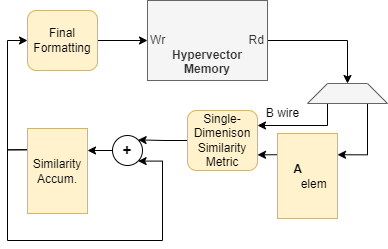
\includegraphics[width=0.3\textwidth]{img/kernel-similarity.png}
    \caption{Architecture of a Single Similarity Kernel}
    \label{fig:sim-kernel}
\end{figure}

The bundling kernel consists of two stages. The initial dimension is first loaded into the bundled element register. Then, for every addition hypervector being bundled, it is loaded from memory, bundled, and accumulated into the bundled element register. When complete, the final bundled vector is written back to the memory.

\begin{figure}[H]
    \centering
    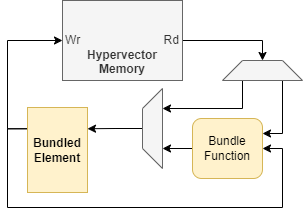
\includegraphics[width=0.3\textwidth]{img/kernel-bundle.png}
    \caption{Architecture of a Single Bundle Kernel}
    \label{fig:bundle-kernel}
\end{figure}

The binding kernel consists of two stages. The initial hypervector is first loaded from the memory into the A\_elem register. Then, the second hypervector is loaded from memory and used with the first in the bind function before being written back to the memory.

\begin{figure}[H]
    \centering
    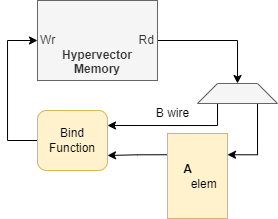
\includegraphics[width=0.3\textwidth]{img/kernel-bind.png}
    \caption{Architecture of a Single Bind Kernel}
    \label{fig:bind-kernel}
\end{figure}

\subsection{System Architecture}

All kernels will share a single hypervector memory. This is both to reduce FPGA area and to allow hypervectors to be bound, bundled, and compared without transferring entire hypervectors between kernel-specific memories. The similarity kernels will also share a dedicated similarity cache to store the results of similarity comparisons. This independent cache was chosen because the result of a similarity comparison is always a single number, not an entire hypervector, and may require a different bit-width than required to store the dimensions of a hypervector.

\begin{figure}[H]
    \centering
    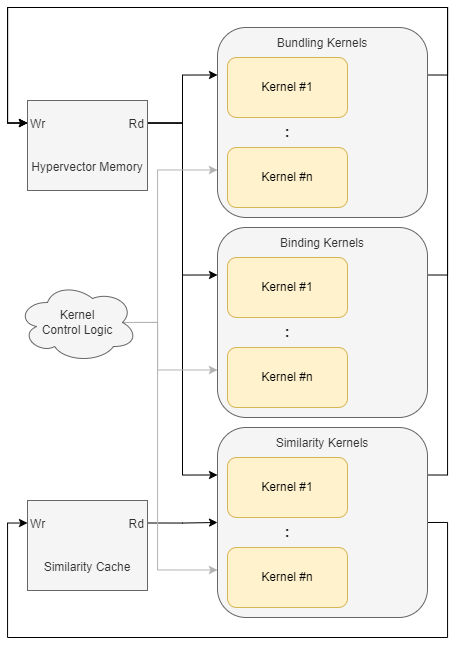
\includegraphics[width=0.3\textwidth]{img/system-level.png}
    \caption{High-Level Archictecture of the Hyperdimensional Computing Accelerator}
    \label{fig:system-level}
\end{figure}

\subsection{AXI Interface}

The AXI interface will expose four registers to the processor. One register will be for loading/storing hypervectors from/to the internal hypervector memory. There will also be registers to initiate hypervector bind, bundle, and similarity operations. Finally, there will be a register to check the status of previously initiated operations. This will be used to ensure the result of an operation only gets used or read elsewhere after it is completed.

\begin{figure}[H]
    \centering
    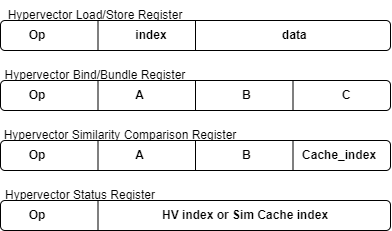
\includegraphics[width=0.3\textwidth]{img/axi-interface.png}
    \caption{Registers Exposed to the Processor by the AXI Interface}
    \label{fig:axi-interface}
\end{figure}

\bibliographystyle{IEEEtran}
\bibliography{references}{}

\end{document}
